\documentclass[12pt]{article}
 
\usepackage[margin=1in]{geometry} 
\usepackage{amsmath,amsthm,amssymb}
\usepackage{float}
\usepackage{tikz}
\usetikzlibrary{arrows,shapes,trees} % loads some tikz extensions
 
\begin{document}
 
\title{Homework 2}
\author{Josh Klontz
CSE 802}
 
\maketitle

\begin{enumerate}
\item \textbf{Solve the following problems from Chapter 2 of the textbook: 8, 10, 14 Parts (a), (b), and (c), 24}
  \subitem \textbf{8. Let the conditional densities for a two-category one-dimensional problem be given by the Cauchy distribution described in Problem 7.}
  \begin{enumerate}
  \item \textbf{By explicit integration, check that the distributions are indeed normalized.}
    \begin{figure}[H]
    \begin{equation}
      p(x|w_i) = \frac{1}{\pi b} \cdot \frac{1}{1 + (\frac{x-a_i}{b})^2}
    \end{equation}
    \caption{Probability density function of a Cauchy distribution.}
    \end{figure}
    The probability density is considered to be normalized if it integrates to 1:
    \begin{equation}
    \begin{split}
      \int_{-\infty}^{\infty} p(x|w_i) dx& = \int_{-\infty}^{\infty} \frac{1}{\pi b} \cdot \frac{1}{1 + (\frac{x-a_i}{b})^2} dx \\
      & = \frac{1}{\pi b} \int_{-\infty}^{\infty} \frac{1}{1 + (\frac{x-a_i}{b})^2} dx
    \end{split}
    \end{equation}
    Apply U-substituion:
    \begin{equation}
    \begin{split}
      u& = \frac{x-a_i}{b} \\
      & = \frac{x}{b} \cdot \frac{a_i}{b} \\
    \frac{du}{dx}& = \frac{1}{b} \\
    dx& = b\ du
    \end{split}
    \end{equation}
    To obtain:
    \begin{equation}
    \begin{split}
      \int_{-\infty}^{\infty} p(x|w_i) dx& = \frac{1}{\pi} \int_{-\infty}^{\infty} \frac{1}{1 + u^2} du \\
      & = \frac{1}{\pi} \cdot tan^{-1}(u) |_{-\infty}^{\infty} \\
      & = \frac{1}{\pi} (\frac{\pi}{2} - \frac{-\pi}{2}) \\
      & = \frac{1}{\pi} \pi \\
      & \boxed{= 1}
    \end{split}
    \end{equation}
  \item \textbf{Assuming that $P(w_1) = P(w_2)$, show that $P(w_1|x) = P(w_2|x)$ if $x = (a_1 + a_2)/2$.}
    \begin{equation}
    \begin{split}
      P(w_1|x)& \iff P(w_2|x) \\
      \frac{p(x|w_1)P(w_1)}{p(x)}& \iff \frac{p(x|w_2)P(w_2)}{p(x)} \\
      p(x|w_1)P(w_1)& \iff p(x|w_2)P(w_2) \\
      p(x|w_1)& \iff p(x|w_2) \\
      \frac{1}{\pi b} \cdot \frac{1}{1 + (\frac{x-a_1}{b})^2}& \iff \frac{1}{\pi b} \cdot \frac{1}{1 + (\frac{x-a_2}{b})^2} \\
      \frac{1}{1 + (\frac{x-a_1}{b})^2}& \iff \frac{1}{1 + (\frac{x-a_2}{b})^2} \\
      1 + (\frac{x-a_1}{b})^2& \iff 1 + (\frac{x-a_2}{b})^2 \\
      (\frac{x-a_1}{b})^2& \iff (\frac{x-a_2}{b})^2 \\
      \frac{x^2-2xa_1+a_1^2}{b^2}& \iff \frac{x^2-2xa_2+a_2^2}{b^2} \\
      x^2-2xa_1+a_1^2& \iff x^2-2xa_2+a_2^2 \\
      -2xa_1+a_1^2& \iff -2xa_2+a_2^2 \\
      -2(\frac{a_1+a_2}{2})a_1 + a_1^2& \iff -2(\frac{a_1+a_2}{2})a_2 + a_2^2 \\
      -(a_1+a_2)a_1 + a_1^2& \iff -(a_1+a_2)a_2 + a_2^2 \\
      (a_1+a_2)a_2 + a_1^2& \iff (a_1+a_2)a_1 + a_2^2 \\
      a_1^2+ a_1a_2 + a_2^2 & = a_1^2+ a_1a_2 + a_2^2 \\
      & \qed
    \end{split}
    \end{equation}
  \item \textbf{Plot $P(w_1|x)$ for the case $a_1=3, a_2=5, b=1$.}
    \begin{equation}
    \begin{split}
      P(w_1|x)& = \frac{p(x|w_1)P(w_1)}{p(x)} \\
      & = \frac{\frac{1}{\pi b} \cdot \frac{1}{1 + (\frac{x-a_1}{b})^2} \cdot 0.5}{\frac{1}{\pi b} \cdot \frac{1}{1 + (\frac{x-a_1}{b})^2} \cdot 0.5 + \frac{1}{\pi b} \cdot \frac{1}{1 + (\frac{x-a_2}{b})^2} \cdot 0.5} \\
      & = \frac{\frac{1}{1 + (\frac{x-a_1}{b})^2}}{\frac{1}{1 + (\frac{x-a_1}{b})^2} + \frac{1}{1 + (\frac{x-a_2}{b})^2}} \\
      & = \frac{1 + (\frac{x-a_2}{b})^2}{1 + (\frac{x-a_1}{b})^2 + 1 + (\frac{x-a_2}{b})^2} \\
      & = \frac{1 + (x-a_2)^2}{2b^2 + (x-a_1)^2 + (x-a_2)^2} \\
      & = \frac{b^2 + (x-a_2)^2}{2b^2 + (x-a_1)^2 + (x-a_2)^2} \\
      & = \frac{1 + (x-5)^2}{2 + (x-3)^2 + (x-5)^2} \\
      & = \frac{x^2 - 10x + 26}{2x^2-16x+36}
    \end{split}
    \end{equation}
    \begin{figure}[H]
      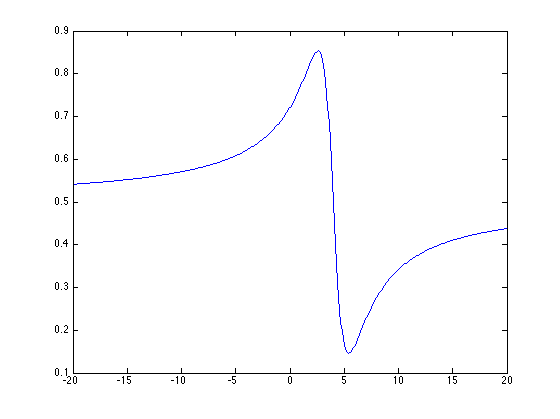
\includegraphics[width=\textwidth]{8c}
    \end{figure}
  \item \textbf{How do $P(w_1|x)$ and $P(w_2|x)$ behave as $x \rightarrow -\infty$ and $x \rightarrow +\infty$? Explain.} \\
    $P(w_1|x)$ and $P(w_2|x)$ approach $\frac{1}{2}$. This is because they have the same variance and their difference in means is decreasingly important as $x \rightarrow \pm \infty$.
  \end{enumerate}
  \subitem{\textbf{10. Consider the following decision rule for a two-category one-dimensional problem: Decide $w_1$ if $x>\theta$; otherwise decide $w_2$.}}
  \begin{enumerate}
  \item \textbf{Show that the probability of error for this rule is given by}
    \begin{equation}
      P(error) = P(w_1)\int_{-\infty}^\theta p(x|w_1)dx + P(w_2) \int_\theta^\infty p(x|w_2)dx
    \end{equation}
    \begin{equation}
    \begin{split}
      P(error)& = \int_{-\infty}^\infty 1-p(w_{decision}|x)dx \\
      & = \int_{-\infty}^\theta 1-p(w_2|x)dx + \int_\theta^\infty 1-p(w_1|x)dx \\
      & = \int_{-\infty}^\theta p(w_1|x)dx + \int_\theta^\infty p(w_2|x)dx \\
      & = \int_{-\infty}^\theta \frac{p(x|w_1)P(w_1)}{p(x)}dx + \int_\theta^\infty \frac{p(x|w_2)P(w_2)}{p(x)}dx \\
      & = P(w_1)\int_{-\infty}^\theta \frac{p(x|w_1)}{1}dx + P(w_2)\int_\theta^\infty \frac{p(x|w_2)}{1}dx \\
      & \boxed{= P(w_1)\int_{-\infty}^\theta p(x|w_1)dx + P(w_2) \int_\theta^\infty p(x|w_2)dx}
    \end{split}
    \end{equation}
  \item \textbf{By differentiating, show that a necessary condition to minimize $P(error)$ is that $\theta$ satisfies}
    \begin{equation}
      p(\theta|w_1)P(w_1)=p(\theta|w_2)P(w_2)
    \end{equation}
    \begin{equation}
    \begin{split}
      \left(P(w_1)\int_{-\infty}^\theta p(x|w_1)dx + P(w_2) \int_\theta^\infty p(x|w_2)dx\right) d\theta& = 0 \\
      P(w_1)\int_{-\infty}^\theta p(x|w_1)dxd\theta + P(w_2) \int_\theta^\infty p(x|w_2)dxd\theta& = 0 \\
      P(w_1)(-p(\theta|w_1)) + P(w_2)(p(\theta|w_2))& = 0 \\
      p(\theta|w_1)P(w_1)& =p(\theta|w_2)P(w_2) \\
      & \qed
    \end{split}
    \end{equation}
  \item \textbf{Does this equation satisfy $\theta$ uniquely?} \\
    No, there may exist multiple values of theta corresponding to multiple optimal decision boundaries based on the underlying probability density functions.
  \item \textbf{Given an example where a value of $\theta$ satisfying the equation actually \emph{maximizes} the probability of error.} \\
    Consider the trivial case where $P(w_1)=P(w_2)$ and $p(x|w_1)=p(x|w_2)$. In this case, all values of $\theta$ maximize the probability of error.
  \end{enumerate}
  \subitem \textbf{14. Consider the classification problem with rejection option.}
  \begin{enumerate}
  \item \textbf{Use the results of problem 13 to show that the following discriminant functions are optimal for such problems:}
    \begin{equation}
      g_i(x) = \left\{ \begin{array}{ll}p(x|w_i)P(w_i) & i = 1, ..., c \\ \frac{\lambda_s-\lambda_r}{\lambda_s}\sum_{j=1}^c p(x|w_j)P(w_j) & i = c+1 \end{array} \right.
    \end{equation}
The optimal desciminant functions maximize the negative risk:
    \begin{equation}
    \begin{split}
      g_i(x)& = \left\{ \begin{array}{ll}-\lambda_s (1-P(w_i|x)) & i = 1, ..., c \\ -\lambda_r & i = c+1 \end{array} \right. \\
      & = \left\{ \begin{array}{ll}-\lambda_s + \lambda_s P(w_i|x)) & i = 1, ..., c \\ -\lambda_r & i = c+1 \end{array} \right. \\
      & = \left\{ \begin{array}{ll}\lambda_s P(w_i|x)) & i = 1, ..., c \\ \lambda_s -\lambda_r & i = c+1 \end{array} \right. \\
      & = \left\{ \begin{array}{ll}P(w_i|x)) & i = 1, ..., c \\ \frac{\lambda_s -\lambda_r}{\lambda_s} & i = c+1 \end{array} \right. \\
      & = \left\{ \begin{array}{ll}\frac{p(x|w_i)P(w_i)}{p(x)} & i = 1, ..., c \\ \frac{\lambda_s -\lambda_r}{\lambda_s} & i = c+1 \end{array} \right. \\
      & = \left\{ \begin{array}{ll}p(x|w_i)P(w_i) & i = 1, ..., c \\ \frac{\lambda_s -\lambda_r}{\lambda_s}p(x) & i = c+1 \end{array} \right. \\
      & \boxed{= \left\{ \begin{array}{ll}p(x|w_i)P(w_i) & i = 1, ..., c \\ \frac{\lambda_s-\lambda_r}{\lambda_s}\sum_{j=1}^c p(x|w_j)P(w_j) & i = c+1 \end{array} \right.}
    \end{split}
    \end{equation}
  \item \textbf{Plot these disciminant functions and the decision regions for the two-category one-dimensional case having}
    \begin{equation}
    \begin{split}
      g_1& = \frac{1}{2\sqrt{2\pi}}e^{-\frac{1}{2}(x-1)^2} \\
      g_2& = \frac{1}{2\sqrt{2\pi}}e^{-\frac{1}{2}(x+1)^2} \\
      g_3& = \frac{g_1 + g_2}{2}
    \end{split}
    \end{equation}
    \begin{figure}[H]
      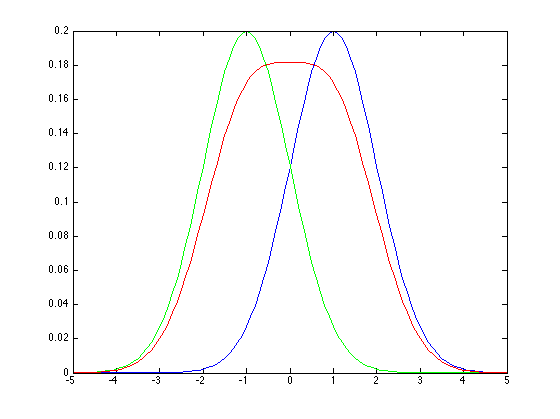
\includegraphics[width=\textwidth]{14b}
      \caption{$g_1 = blue$, $g_2 = green$, $g_3 = red$. Decision boundaries at $g_1 = g_3$ and $g_2 = g_3$.}
    \end{figure}
  \item \textbf{Describe qualitatively what happens as $\lambda_r/\lambda_s$ is increased from 0 to 1.} \\
  When $\lambda_r/\lambda_s = 0$ there is no cost associated with the rejection option and it should be taken every time. As $\lambda_r/\lambda_s$ increases, the size of the $g_3$ distribution shrinks with respect to $g_1$ and $g_2$, and the decision region where the rejection option should be taken becomes increasingly narrow. When $\lambda_r/\lambda_s = 1$ there is no instance where it is optimal to take the rejection option.
  \end{enumerate}
\end{enumerate}
 
\end{document}
